\chapter{Results}
show all views results.
differece of this shader compared to evaluation shader
show real snake images for comparison with real rendered images
show experiments received
show rendered images by daljits implemetation of stams approach.
show our renderer's results 
mention all input parameters and their values.
mention system specs and how long it took in order to precompute
show some idft2 images, used patch, besids rendered image
what initial size was used patch?
mention GEM results.
mention real results from geneva - use same paramter setup.

\section{Other stuff}
$\forall \colvec[x]{y}{z} \in \mathbb{R}^3 : \exists r \in [0,\infty) \exists \phi \in [0,2\pi] \exists \theta \in [0,\pi] $ s.t.
\begin{equation*}
\colvec[x]{y}{z} = \colvec[r sin(\theta)cos(\phi)]{r sin(\theta)sin(\phi)}{r cos(\theta)}
\end{equation*}

\section{Matlab code}
\section{Discussion}


\begin{figure}[ht]
  \centering
  \subfigure[Blaze grating]{
    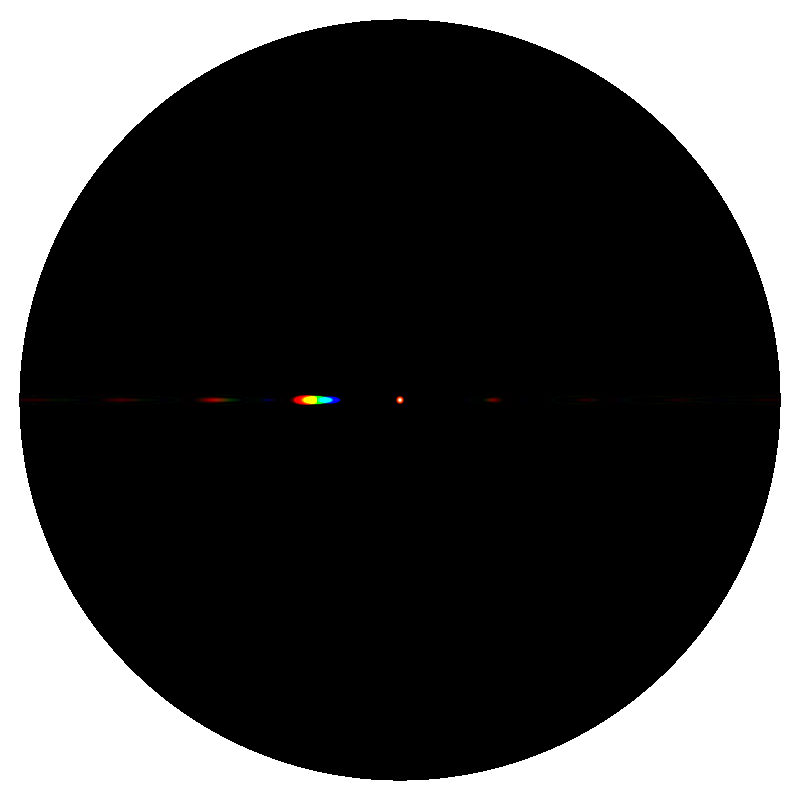
\includegraphics[scale=0.12]{results/diffPatches/fftBlazeHeight_0.25Microns_allL_weak_scale.png}
    \label{fig:brdfmapBlaze}
  }
~
  \subfigure[elaphe grating]{
    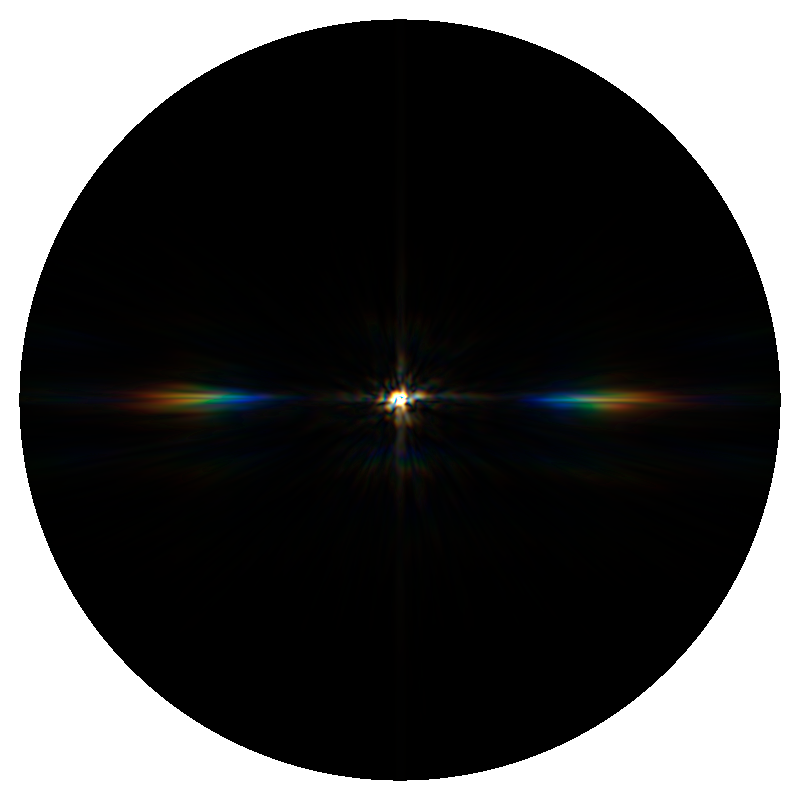
\includegraphics[scale=0.12]{results/diffPatches/elaph65.png}
    \label{fig:brdfmapElaphe}
  }
~
  \subfigure[xeno grating]{
    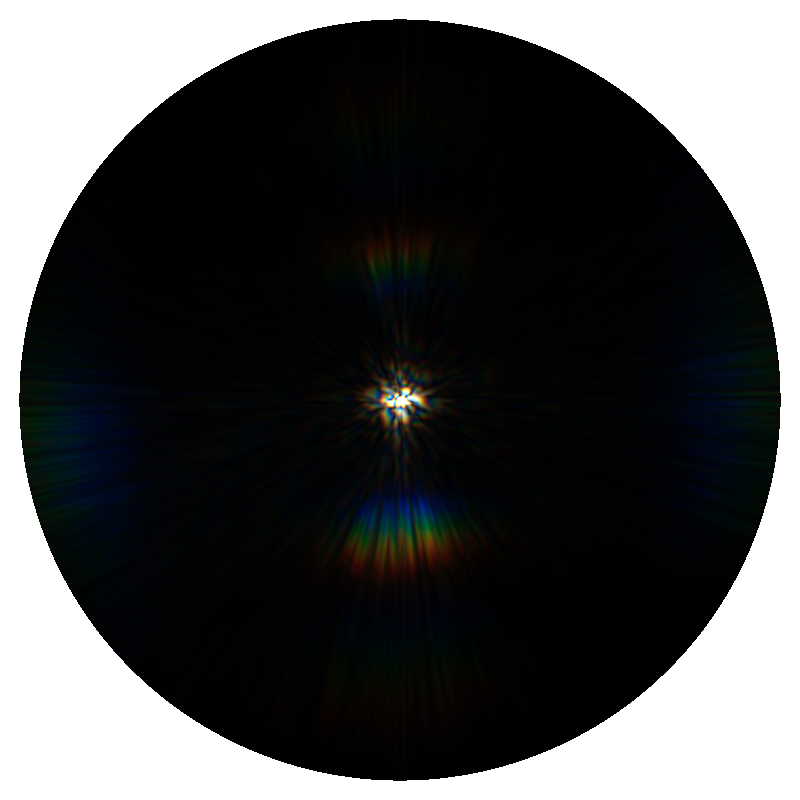
\includegraphics[scale=0.12]{results/diffPatches/xeno65.png}
    \label{fig:brdfmapXeno}
  }
  \label{brdfmapsDiffPatches}
  \caption{BRDF maps for different patches}
\end{figure}


\begin{figure}[ht]
  \centering
  \subfigure[$\lambda_{step=1 nm}$]{
    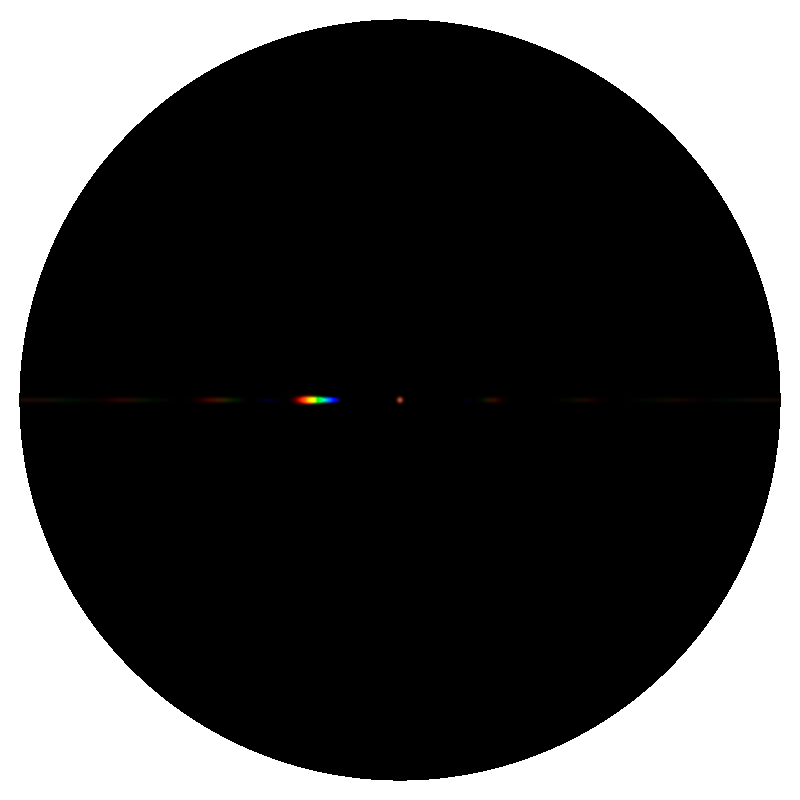
\includegraphics[scale=0.12]{results/different_lambda_steps/blaze/dl=1.png}
    \label{fig:brdfmapsDiffLambdaStepsL1BlazeL}
  }
~
  \subfigure[$\lambda_{step=5 nm}$]{
    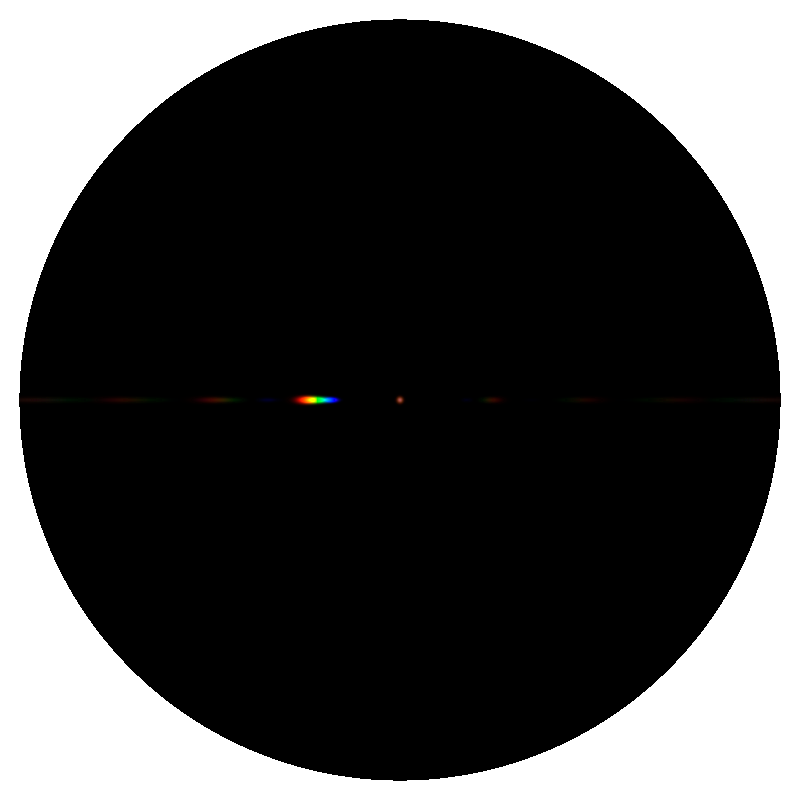
\includegraphics[scale=0.12]{results/different_lambda_steps/blaze/dl=5.png}
    \label{fig:brdfmapsDiffLambdaStepsL5Blaze}
  }
~
  \subfigure[$\lambda_{step=10 nm}$]{
    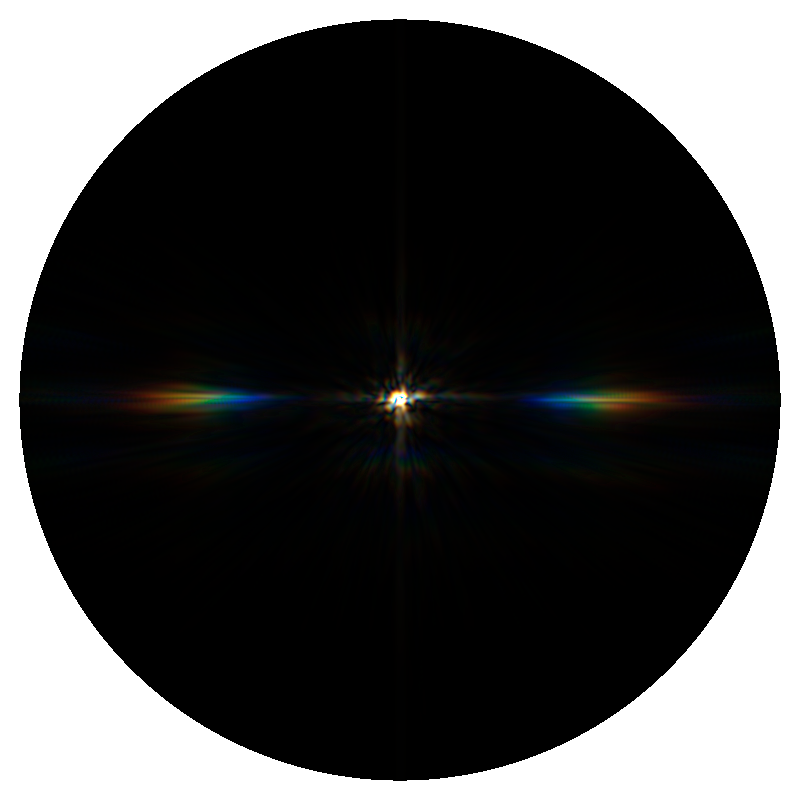
\includegraphics[scale=0.12]{results/different_lambda_steps/blaze/dl=10.png}
    \label{fig:brdfmapsDiffLambdaStepsL10Blaze}
  }
  
  \subfigure[$\lambda_{step=25 nm}$]{
    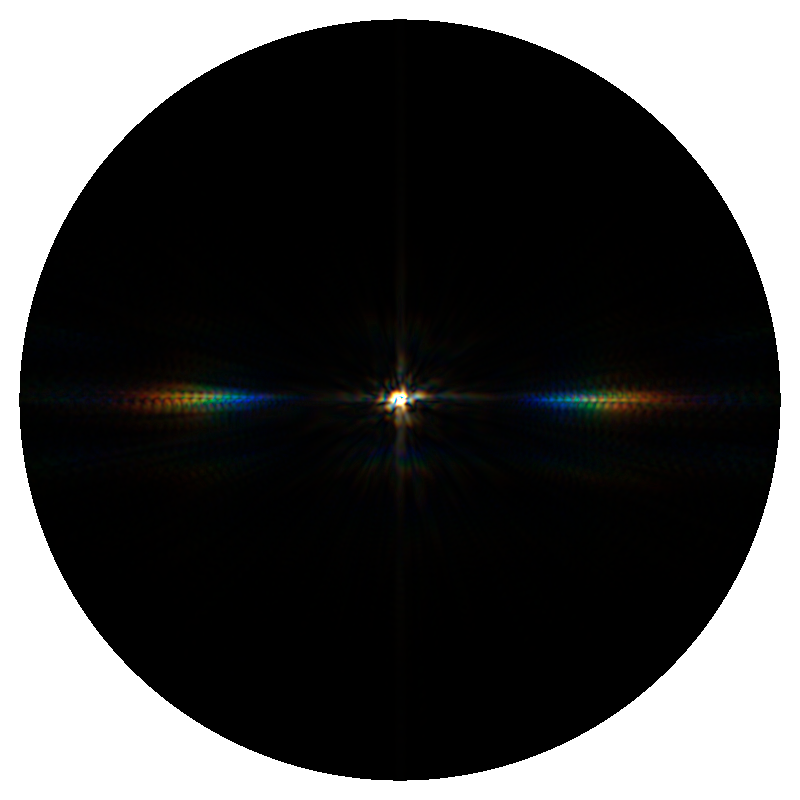
\includegraphics[scale=0.12]{results/different_lambda_steps/blaze/dl=25.png}
    \label{fig:brdfmapsDiffLambdaStepsL25Blaze}
  }
~
  \subfigure[$\lambda_{step=50 nm}$]{
    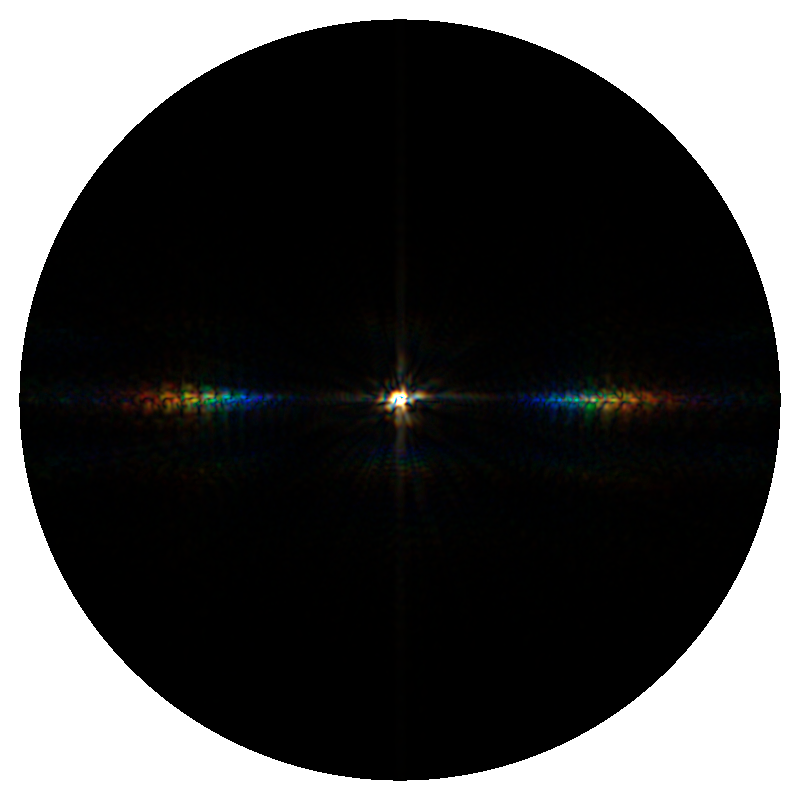
\includegraphics[scale=0.12]{results/different_lambda_steps/blaze/dl=50.png}
    \label{fig:brdfmapsDiffLambdaStepsL50Blaze}
  }
~ 
  \subfigure[$\lambda_{step=100 nm}$]{
    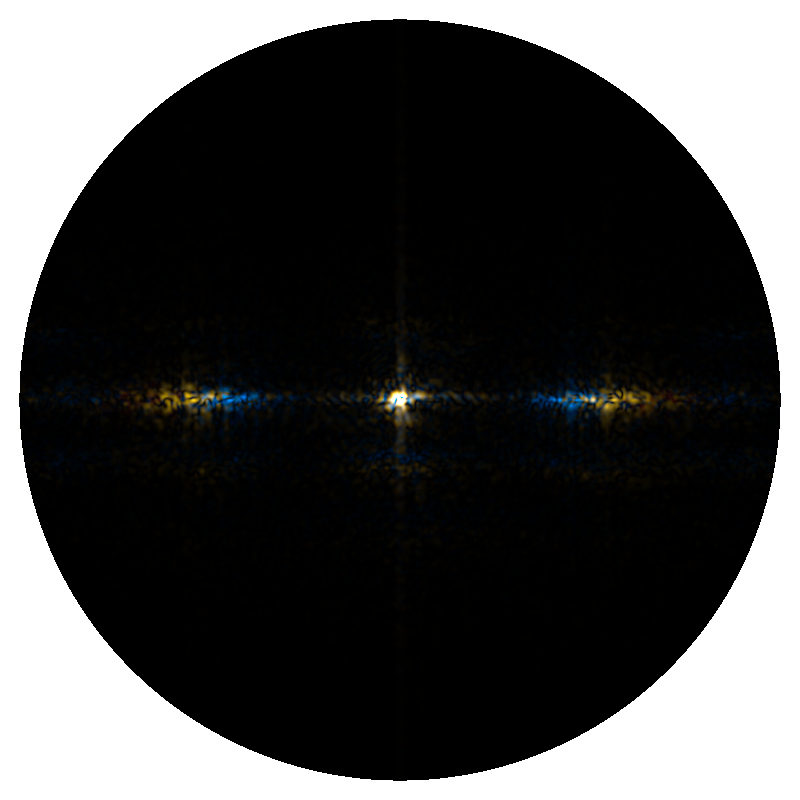
\includegraphics[scale=0.12]{results/different_lambda_steps/blaze/dl=100.png}
    \label{fig:brdfmapsDiffLambdaStepsL100Blaze}
  }
  
  \label{brdfmapsDiffLambdaStepsBlaze}
  \caption{Blaze grating: Different lambda step size}
\end{figure}


